\documentclass[a4paper,11pt]{kth-mag}
\usepackage[pdftex]{graphicx}
\usepackage[T1]{fontenc}
\usepackage{textcomp}
\usepackage{lmodern}
\usepackage[utf8]{inputenc}
\usepackage[swedish,english]{babel}
\usepackage{modifications}
\usepackage[retainorgcmds]{IEEEtrantools}
\usepackage{amsmath}
\usepackage{amsthm}
\usepackage{amssymb}
\usepackage{amsfonts}

\usepackage{clrscode}
\usepackage{hyperref}
\usepackage{graphicx}
\usepackage{tikz}
\usepackage{pgfplots}

\graphicspath{
        {figures/}
        {figures/smiley/}
        {figures/mp-graph/}
        {figures/hmm-graph/}
        {figures/hmm-pf-graph/}
        {figures/gwhisker_database/}
        {figures/gwhiskers/}
        {figures/COD/}
        {figures/response/}
        }

\theoremstyle{definition}
\newtheorem{definition}{Definition}
\newtheorem{example}{Example}
\newtheorem{theorem}{Theorem}
\newtheorem{note}{Note}

\newcommand{\ForEach}{\textbf{for each} }
\newcommand{\In}{\textbf{in} }
\newcommand{\Spline}[2][a]{#1_3#2^3 + #1_2#2^2 + #1_1#2}

\newcommand{\NN}{\ensuremath{\mathbb{N}}}
\newcommand{\ZZ}{\ensuremath{\mathbb{Z}}}
\newcommand{\RR}{\ensuremath{\mathbb{R}}}
\newcommand{\CC}{\ensuremath{\mathbb{C}}}
\newcommand{\HS}{\ensuremath{\mathcal{H}}}
\newcommand{\IS}{\ensuremath{\mathcal{I}}}
\newcommand{\XS}{\ensuremath{\mathcal{X}}}
\newcommand{\ZS}{\ensuremath{\mathcal{Z}}}
\newcommand{\TS}{\ensuremath{\mathcal{T}}}

%operators
\newcommand{\abs}[1]{\left\vert #1 \right\vert}
\newcommand{\argmax}[1]{\underset{#1}{argmax}}
\newcommand{\argmin}[1]{\underset{#1}{argmin}}

\newcommand{\prob}[1]{p{(#1)}}
\newcommand{\cprob}[2]{\prob{\left. #1 \middle\vert #2 \right.}}
\newcommand{\cprobnext}[1]{\cprob{#1_t}{#1_{t-1}}}
\newcommand{\ndist}[2]{\mathcal{N}{\left(#1, #2\right)}}
\newcommand{\norm}[1]{\left\vert\left\vert#1\right\vert\right\vert}
\newcommand{\Lp}[1][p]{\mathrm{L}^{#1}}
\newcommand{\Lpnorm}[2][p]{\norm{#2}_{\Lp[#1]}}

\newcommand{\Response}[3]{\langle #1, #2\rangle_{#3}}


\newcommand{\Ordo}[1]{\mathcal{O}{\left(#1\right)}}

\newcommand{\xtmN}[4]{
  \left\{#1_{#2}^{#3}\right\}_{#3=1}^{#4}
}
\newcommand{\interval}[2]{
  \left[#1, #2\right]
}
\newcommand{\bel}[1]{
  bel\left(#1\right)
}

\newcommand{\tf}{x_{\text{from}}}
\renewcommand{\tt}{x_{\text{to}}}
\newcommand{\trans}{\left( \tf, \tt \right)}
\newcommand{\coeffs}{\left( a_3, a_2, a_1 \right)}

\title{
    Probabilistic Tracking of Multiple Rodent Whiskers in Monocular Video
    Sequences\\ <SECOND DRAFT>
}

\subtitle{
    A small step towards cheap, reliable, and non-intrusive automatic tracking of whiskers.
}
\foreigntitle{
    Statistisk Följning av Multipla Morrhår på Gnagare i Video.
}
\author{
    Jim Holmström\\
    \href{mailto:jimho@kth.se}{jimho@kth.se}\\
    Emil Lundberg\\
    \href{mailto:emlun@kth.se}{emlun@kth.se}
}
\date{May 2012}
\blurb{
  SA104X Examensarbete inom teknisk fysik, grundnivå\\
  Bachelor's Thesis at CSC, KTH\\
  Supervisor: Prof. Örjan Ekeberg\\
  Examiner: Prof. Örjan Ekeberg
}
\trita{TRITA xxx yyyy-nn}
\begin{document}
\frontmatter
\pagestyle{empty}
\removepagenumbers
\maketitle
\selectlanguage{english}
\begin{abstract}
    The interest in studying rodent whiskers has recently seen a significant increase, particularly in the field of neurophysiology. As a result, there is a need for automatic tracking of whisker movements. Currently available commercial solutions either are extremely expensive, place great restrictions on the experiment, or fail when whiskers cross or overlap.

This thesis proposes a proof-of-concept implementation of a probabilistic tracking system. This solution uses a technique known as the \emph{Particle Filter} to propagate a whisker model between frames of high speed video. In each frame, the next state of the model is predicted by comparing the model with a database of training data.

The main strengths of the proposed solution is that it successfully tracks multiple whiskers at once, even when they cross or overlap, and does not notably restrict the experiment. However, it is not yet accurate enough for the intended use.

----

The purpose for this thesis is to implement an mockup of an portable 
program capable of reilably tracking multiply rodent whiskers 
in good conditioned video and to evaluate different mathematical 
models for the whiskers and snout. 

The backbone algorithm used 
for tracking is the particle filter which works on statistical basis which
is used for the purpose of refinding the object closeby it's last known location
and to reduce the complexity for the search down to feasible values.

\end{abstract}
\clearpage
\begin{foreignabstract}{swedish}
    
Intresset för att studera morrhår på gnagare har på senare tid
ökat, speciellt inom neurofysiologin.  Som ett resultat av detta
finns det ett behov av automatisk följning av morrhår.  Nuvarande
kommersiella lösningar är antingen extremt dyra, sätter
begräsningar på experimentuppställningen eller misslyckas i
stökiga miljöer eller när överlappning förekommer.

Denna avhandling bidrar med en enkel implementation av ett
\emph{probabilistiskt} följningssystem.  Lösningen använder sig av
en teknik som kallas \emph{partikelfilter} för att propagera en
morrhårmodell mellan bildrutor i höghastighetsvideo.  För varje
bildruta förutspås nästa tillstånd genom att fråga en förtränad
\emph{databas} och filtera svaret genom partikelfiltret.
Implementationen är skriven i Python 2.6 och använder sig av
programbiblioteken NumpPy och SQLite3.

Testresultaten indikerar att metoden är rimlig.  Med endast en grovt
snarlik databas lyckades algoritmen följa multipla morrhår, dock
endast under korta sekvenser i taget.  Bättre träningsdata, såsom
handmarkerad riktig data, skulle kunna förbättra resultatet
väsentligt.


\textbf{Nyckelord:} Följning, Multipla, Morrhår, Partikelfilter,
Övergångsdatabas, Modelevaluering, Proof-of-Concept

\end{foreignabstract}
\clearpage
\tableofcontents*
\mainmatter
\pagestyle{newchap}
\chapter{Introduction}
    \label{sec:introduction}
    \subsection{Background and problem formulation}

- Video tracking (finding) is interesting
- Biologists want to track the movements of animals or parts of animals
- Most of the software available for this purpose is expensive
- Most of the software available cannot handle too many whiskers at once (clutter)
- Hedvig developed a way to track human motion in 3d using monocular video
- We want to use the ~ the same method for tracking whiskers (different mechanical model)
- What do ekeberg want and why?

KEYWORDS
- Spatial/temporal resolution

With the ever increasing power and mobility of computers, the concept of computer vision has recently seen a large increase in interest. Encompassing problems such as classification, recognition, perception and tracking, ...

In particular, biology and neuroscience researchers are interested in tracking the movements of animals or parts of animals. One such field aims to study the movements of rodent whiskers, including how they are used for perception and their correlation with neural signals. However, most whisker tracking software available today suffers a few fundamental flaws. First and foremost, they are often so expensive that not even well funded laboratories feel they can afford them. Cheaper solutions often have problems with tracking multiple whiskers at once, often requiring removal of almost all whiskers. Even if the rodent adapts to the change, it may introduce systematic errors. Some higher precision systems impose other restrictions on the experiment, such as restraining the animal or attaching motion capture markers to the whiskers, which may also cause systematic errors and not give a representative view of how the animal naturally uses the whiskers.

In general, the main difficulty in tracking and localization is to separate the object from clutter such as (...), occlusion (...), and (fill the list). (Hedvig here?) In the case of whisker tracking, the dominant problems are that whiskers often overlap and vary in size.

In 2001, Hedvig Sidenbladh developed a probabilistic method for tracking three-dimensional human motion in monocular video. This method deals with many of the problems inherent in computer vision

(Vad Hedvig introducerat som e najz) The goal of this project is to apply the same kind of method used by Sidenbladh to tracking whiskers. We will investigate whether this is feasible, and if it is we will try some different tracking models and see how they perform.



\chapter{Related Work}
    \label{sec:related_work}
    The following is a summary of some of the work that has been done in
the field of automatic whisker tracking, as well as a Ph.D thesis on
probabilistic tracking of human motion. The work in this thesis will
be based on the latter, being a similiar - though a lot simpler -
solution applied to the case of whisker tracking.


\subsection{High-Precision, Three-Dimensional Tracking of Mouse
  Whisker Movements with Optical Motion Capture Technology}

\cite{BadExample1} describes a whisker tracking system that uses
motion capture markers and two tracking cameras to track whisker
movements in 3D. A spatial resolution of $<0.5$ mm in all dimensions
and a temporal resolution of $5 ms$ is reported. The impact of the
markers on whisker movements were investigated by comparison with a
light beam detection system, and no significant difference was
detected. The system requires head fixation since the markers need to
be visible to both cameras at all times.
        

\section{Unsupervised Whisker Tracking in Unrestrained Behaving
  Animals}

\cite{UnsupervisedTracking} provides a solution that uses
frame-by-frame image analysis of off-line monocular images, and does
not impose other restrictions on the setup. The solution is based on
creating vector fields using anisotropy in the image and tracks
movements along the full length of the whiskers. It is fully
automatic, and successfully tracks up to 8 whiskers on each side of
the snout simultaneously, though it suffered some difficulties when
applied on full whisker arrays.


\section{Probabilistic Tracking and Reconstruction of 3D Human Motion in Monocular Video Sequences\cite{Hedvig}}
    




\chapter{Definitions}
    \label{sec:definitions}
    %TODO 
%\section{Invariances}
%Section about invariances and why they are needed in localization.

%The "filter" must give the same response invariant of the position in the image 
%and its often wanted to have it rotational and scale invariant (if your not 
%intending to measure things like angles or size that is)

\section{Data}
\subsection{Image}
In a computer an \emph{image} is represented as an array of numbers, mostly 8bit integers ranging between $\left[0,255\right]$ 

\subsubsection{RGB image}
A color image can be defined as
\begin{equation}
    \begin{array}{ccc}
    RGBimage : \NN^2 &\rightarrow& \NN^3\\
    RGBimage : position&\rightarrow&color
    \end{array}
\end{equation}
Which basically is foreach position in the image we have a response color.
An alternitve represenation whould be $\NN^5=\langle pos,value\rangle$.

The RGB image space is denoted by
\begin{equation}
    RGBimage\in \IS_{RGB}
\end{equation}

\subsubsection{Grayscale image}
A grayscale image can, similary to RGB images, be defined as a function
\begin{equation}
    \begin{array}{ccc}
    I : \NN^2 &\rightarrow& \NN\\
    I : position&\rightarrow&intensity
    \end{array}
\end{equation}
or alternatively $\NN^3=\langle pos,intensity\rangle$.

Finally the $image$-space is denoted by
\begin{equation}
    I \in \IS
\end{equation}

\begin{example}~\\
    \begin{tabular}{lcr}
        $
        \begin{pmatrix} 
        255&  255&  255&  255&  255&  255&  255&  255&  255&  255\\
        255&  255&  255&  255&  255&  255&  255&  255&  255&  255\\
        255&  255&  255&    0&  255&  255&    0&  255&  255&  255\\
        255&  255&  255&    0&  255&  255&    0&  255&  255&  255\\
        255&  255&  255&  255&  255&  255&  255&  255&  255&  255\\
        255&    0&  255&  255&  255&  255&  255&  255&    0&  255\\
        255&  255&    0&  255&  255&  255&  255&    0&  255&  255\\
        255&  255&  255&    0&    0&    0&    0&  255&  255&  255\\
        255&  255&  255&  255&  255&  255&  255&  255&  255&  255\\
        255&  255&  255&  255&  255&  255&  255&  255&  255&  255
        \end{pmatrix}
       $
       &$\Rightarrow$& \parbox[c]{1em}{
\includegraphics[scale=10.0]{smiley.png}}
    \end{tabular}
\end{example}

\subsubsection{Video}
A \emph{video} can be represented as a function mapping an integer to the designated image $I$
\begin{equation}
    video : \NN \rightarrow I
\end{equation}

\subsection{State}
<intro about state>
\begin{note}
    State and hypothesis is model dependant.
\end{note}
\subsubsection{State}
$x$
\subsubsection{State-space}
$x\in\XS$ %TODO(collides with X?)
\subsubsection{Hypothesis}
$z$

Explain: Hypotesis (in the context of PF), sample, DOF?, 

\subsubsection{Hypothesis-space}
$z\in\ZS$

\subsubsection{Estimate}
The algorithms estimate of the ground truth
$x^*$ 

\subsubsection{Degrees of Freedom (DOF}
The number of adjustable parameters in a model.

\subsubsection{Observation}
<placement?><denotation?>

\subsection{MISC?}

\subsubsection{Prop. function as a collection of points with attached weight.}

\subsubsection{Dynamic system}
    It's a tuple <space,update,time>
    Any mechanical system following newton physics (or relativistic for that matter) can be considered to be an dynamic system
    in our case the tuple whould be <feature\_space,update\_rule (the one we are trying to preprocess data to approximate),time>



\chapter{Theory}
    \label{sec:theory}
    \newcommand{\xtmN}[4]{
  \left\{#1_{#2}^{#3}\right\}_{#2=1}^{#4}
}
\newcommand{\interval}[2]{
  \left[#1, #2\right]
}
\newcommand{\bel}[1]{
  bel\left(#1\right)
}

\subsection{The particle filter}
\subsubsection{Introduction}
The core of tracking engine used is a technique known as the \emph{particle filter}. The particle filter is a kind of Bayesian filtering where one uses discrete hypotheses to approximate continuous probability distributions \cite{ProbRob}. The main idea can be outlined as follows.

Suppose we have a system described by the state $x_t$ at time $t$. $x_t$ can be thought of as a vector of state parameters. Suppose that we know the previous state $x_{t-1}$ and have an observation $z_t$ of the system at the current time. In general, it is difficult to accurately determine $x_t$ from the observation alone, and the observation may suffer from interference. Therefore, we cannot directly read $x_t$ from $z_t$. However, we can estimate $x_t$ if we know the following things about the system:

\begin{itemize}
\item A probability function $p$, where $p\left(x_t | x_{t-1}\right)$ is the probability that the current state is $x_t$ if the previous state was $x_{t-1}$.
\item A probability function $q$, where $q\left(z_t | x_t\right)$ is the probability that we observe $z_t$ if the current state is $x_t$.
\end{itemize}

Using $p$ and knowing $x_{t-1}$, we can generate a set of hypotheses $\xtmN{\bar{x}}{t}{m}{N}$ for the current state $x_t$. Using $q$ and knowing $z_t$, we can evaluate how likely the hypotheses are. If it is likely to observe $z_t$ if the current state is $x_t$, then $x_t$ is probably a good estimate of the current state. With this information, we select the most probable hypotheses and let them be our estimate of the current system state.

The particle filter works recursively in two steps:

\begin{enumerate}
\item The \emph{sampling step} is the generation of the hypotheses, known as \emph{particles}, from the previous state $x_{t-1}$. The belief $\bel{x_{t-1}}$, see below, is used as an estimate for $x_{t-1}$. What makes this recursive is the fact that $\bel{x_t}$ is calculated using $\bel{x_{t-1}}$.

\item The \emph{resampling step} is the final selection of the most probable particles. After resampling the set $\bar{X_t} := \xtmN{\bar{x}}{t}{m}{N}$ we get the \emph{belief} $\bel{x_t}$, which often includes multiple copies of the most probable particles. This set is used as an estimate for $x_t$, and is used to estimate $x_{t+1}$.
\end{enumerate}

In the next section, the particle filter algorithm will be stated. Implementing the filter in itself is only a matter of implementing the stated pseudocode, and is not difficult. The difficult part is designing the probability functions $p$ and $q$ for the given system. A probabilistic implementation of these functions is proposed in chapters TODO.


\subsubsection{Formal description of the particle filter}
Here the particle filter algorithm is stated. An elaboration on what this actually does and why is offered below.
%TODO pseudo algorithm for the 
%Sample instead of draw

\begin{codebox}
\Procname{$\proc{Distribution-Sample}(X_t,p)$}
\li \ForEach $\id{x_t}$ \In $\id{X_t}$
\li     \Do
            $sample \id{x_{t+1}} \sim p\left(x_{t+1}|x_t\right)$
        \End
\li \Return $\id{X_{t+1}}$
\end{codebox}
\begin{codebox}
\Procname{$\proc{Importance}(X,q,z)$}
\li \ForEach $\id{x}$ \In $\id{X}$ 
\li     \Do
            $w \gets q\left(z|x\right)$
        \End
\li \Return $W$
\end{codebox}
\begin{codebox}
\Procname{$\proc{Weighted-Sample}(X,W)$}
\li \ForEach $x$ \In $X$
\li     \Do
            $sample ~ x' \propto W$   
        \End
\li \Return $X'$
\end{codebox}
\begin{codebox}
\Procname{$\proc{Particle-Filter} (X_{t-1},z_t)$}
\li $X_t \gets \proc{Distribution-Sample}(X_{t-1},p)$
\li $W_t \gets \proc{Importance}(X_{t-1},q,z_t)$
\li $X_t \gets \proc{Weighted-Sample}(X_t,W_t)$
\li \Return $X_t$
\end{codebox}

\begin{codebox}
\Procname{$\proc{Particle-Filter} (X_{t-1}, z_t)$}
\li Let $\bar{X_t} = \emptyset$.
\li For $m:=1$ to $\left|X_{t-1}\right|$:
\li \Do Draw $x_t^m$ with probability $p\left(x_t^m | x_{t-1}^m\right)$.
\li Let $w_t^m := q\left(z_t | x_t^m\right)$.
\li Add $(x_t^m, w_t^m)$ to $\bar{X_t}$.
\End
\li Let $X_t := \emptyset$.
\li For $m:=1$ to $\left|X_{t-1}\right|$:
\li \Do
    Draw $x_t^m$ with probability proportional to $w_t^m$
    \li Add $x_t^m$ to $X_t$.
    \End
\li Return $X_t$.
\end{codebox}


We draw a set $\bar{X}_t = \xtmN{x}{m}{t}{N}$ of samples from $p$. These samples roughly represent a probability distribution for the current state $x_t$, but we have yet to consider our observation. Therefore, we will create a new probability distribution weighted by how probable the observation $z_t$ is. For each $x_t^m$, we let $w_t^m := q\left(z_t | x_t\right)$. This defines a discrete probability distribution where $x_t^m$ is assumed with a probability proportional to $w_t^m$. From this final distribution we again draw $N$ samples $X_t$, which will be our estimate of the current state. The elements $x_t^m$ are referred to as \emph{particles} and the set $X_t$ as the \emph{belief at time $t$}.

In this thesis, $x_{t-1}$ is not known. Rather $x_{t-1}$ is estimated with a set $X_{t-1}$ of $N$ particles. In this case, $x_t^m$ is sampled with probability $p\left(x_t^m | x_{t-1}^m\right)$.



\subsubsection{Curse of dimensonality}
The 8 DOF in our model produces vast amounts of space in our feature space and this has the consequence that we need proportional to $n^8$ datapoints to fill it to an specified density c.

For instance, we would need $4^8=65536$ samples just to make a grid with 4 samples in each DOF which in many cases (aspecially for hand labeled data). 

This phenomen of having hue searchspace in highdimensinonal space is fairly common and have the name "Curse of dimensionality".

One way to somewhat overcome this emptyness in space is to have a dynamic (active?) algorithm that adopts the sample density 
according to the models relative frequency in that area and this results in, for a given amount of samples, its more likely 
for an sampled model to occure in a more densly pre-sampled (pre-sampled?) area, in fact this method when doing it right (ideally) 
gives: given a set of samples the overall density for all the samples in the sampledatabase would be optimal) [proof for this will be given in <blabla>]
... (use the world hypotesis instead of sample, or perhaps sampled-hypotesis)
(below is perhaps somewhat redudant, but one can pick bits and pieces from both)
So having a bias towards trying out more plausible hypotesis for the models innerstate is better than 
doing a naive exhausted search tru the entire feature space, this could only be used if you have $\le$ 3 DOF as in for example finding straight edges with houghtransformation[ref].
...
One method that uses prior knowledge of the models PDF and a pretrained database containing knowledge on how to approximate the models PDF in the next timestep is particle filter which is an (instance?) of the ideal bayesian filter.






\subsection{Particle filtering whisker movements}
Here we propose a way to model whiskers as a dynamic system.

\subsection{Kinematic whisker models}

In all our models we have separated the head from the whiskers since they have
such different kinematic properties and actually are attached to each other.

==The first model
Assumptions:
>Material is linear elastic
>Small deformations (probably the biggest assumption, which dont actually hold
in our case)

The equation of elastic line ... [Grundläggande Hållfasthetslära - Hans Lundh
p94 (7.6)]

The force that comes from the head moving on the base of the whisker is just 
sucked up by the Boundaryvalues and it will still be valid assumptions for the
elasticline to hold.

Under just a few assumptions that the material is linear elastic and the
deformations are small we have the ...


============== MODELS =================

One possible model is to borrow the model for beam under small 
deformations from the theory of strength of materials,
after all the whisker is a beam but we dont have small 
deformations at all but we assume that the model will approximatly hold ony way.




\chapter{Algorithms and Implementations}
    \label{sec:algorithms_implementations}
    \subsection{The particle filter}

\subsection{The state transition database}




%TODO results or Results?
%TODO does one write benchmarking? and results?
\chapter{Results}
    \label{sec:benchmarks_results}
    The results consist of three main parts:
\begin{itemize}
\item A benchmark of the impact of different parameters on the
  tracking performance, performed on synthetic videos and evaluated
  programmatically
\item Test runs on real data with the best performing parameters from
  the benchmark, evaluated manually
\item Conclusions concerning the feasibility of a probabilistic
  whisker tracking system.
\end{itemize}

\section{Parameter Benchmark}

A benchmark was performed in order to identify how tracking
performance is affected by the different parameters. The benchmark was
performed on generated videos of synthetic whiskers, which enabled
programmatic evaluation of the results since the correct shapes of the
whiskers were known.

\subsection{Test data}
\label{sec:test-data}

The test data consisted of a single generated video of synthetic
whiskers. The video contained 6 whiskers and was 64 frames long. Each
whisker had length 200 and a random base shape $\Spline{\omega}$, with
$a_3, a_2, a_1$. Each $a_i$ was in the range $\left[0,
  \sigma_i\right)$, where $\sigma_3 = 1.6 \cdot 10^{-5}, \sigma_2 =
4\cdot 10^{-3}, \sigma_1 = 1$. Each whisker was then assigned a random
phase $d \in \left[0, 2\pi\right)$, and the shape at time step $t$ was
$\left(\Spline{\omega}\right) \sin(\frac{2\pi t}{30} + d)$. The
frequency $\frac{1}{30}$ was selected through manual inspection of a
video of real whiskers. The resulting whiskers were roughly
reminiscent of real whiskers, and 6 sample frames can be seen in
figure \ref{fig:benchmark-video}.

The database was generated with the same parameters, and contained
$2^{14} = 16384$ transitions. Each transition consisted of a ``from''
part $\tf$ and a ``to'' part $\tt$. $\tf$ was created by generating a
base state and phase in the same way as for the video, and setting
$t=0$. $\tt$ was created by taking $\tf$ and increasing the phase by
$\frac{2\pi}{30}$.

\begin{figure}
  \centering
  \begin{tabular}{ccc}
    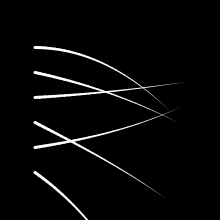
\includegraphics[width=0.3\textwidth]{benchmark-video/frame-00000.png} &
    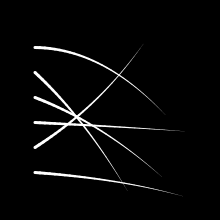
\includegraphics[width=0.3\textwidth]{benchmark-video/frame-00005.png} &
    
\includegraphics[width=0.3\textwidth]{benchmark-video/frame-00010.png}\\
    Frame 0 & Frame 5 & Frame 10\\
    
\includegraphics[width=0.3\textwidth]{benchmark-video/frame-00015.png} &
    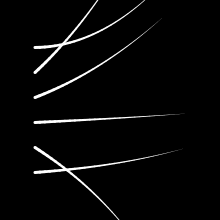
\includegraphics[width=0.3\textwidth]{benchmark-video/frame-00020.png} &
    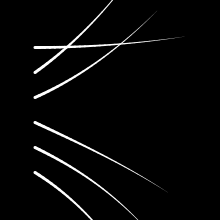
\includegraphics[width=0.3\textwidth]{benchmark-video/frame-00025.png}\\
    Frame 15 & Frame 20 & Frame 25
  \end{tabular}
  \caption{Sample frames from the testing video.}
  \label{fig:benchmark-video}
\end{figure}  


\subsection{Evaluated parameters}
The following parameters were evaluated:

\begin{description}
\item[n] Number of particles
\item[p] In which $\Lp$ space to compute $\Lpnorm{\tf - x_{t-1}}$ in
  the prediction step
\item[a] The exponent for the weights in the prediction step, $w =
  \left(\Lpnorm{\tf - x_{t-1}}\right)^{-a}$
\item[$\sigma$] Standard deviation modifier for the offset in the
  prediction step. Standard deviations for the $\omega^3, \omega^2$
  and $\omega$ terms are $0.1\sigma\sigma_3, 0.1\sigma\sigma_2$ and
  $0.1\sigma\sigma_1$, respectively.\footnote{See section
    \ref{sec:test-data} for the $\sigma_i$ values.}
\item[g] The exponent for the importance in the filtering step
\end{description}

Table \ref{tbl:testcases} shows the tested values.

\begin{table}
  \centering
  \begin{tabular}{c|l}
    Parameter & Values\\
    \hline
    $n$ & 64, 128, 256, 512\\
    $p$ & 2, 4, 8\\
    $a$ & 1, 2, 4, 8\\
    $\sigma$ & 0.25, 0.5, 1, 2\\
    $g$ & 1, 2, 4, 8
  \end{tabular}
  \caption{Specification of test cases.}
  \label{tbl:testcases}
\end{table}

\subsection{Benchmark procedure}

The benchmark was run on the test video for each combination of
parameters in table \ref{tbl:testcases}. The output from the benchmark
is an error tensor $\epsilon_{i,t}$, where index $i, t$ contains
$\Lpnorm[2]{Z_t - x_t}$, the $\Lp[2]$ distance between the ground
truth and estimated shape for whisker $i$ at time $t$. From this a
list $\epsilon_i$ was computed as the root mean square of
$\epsilon_{i,t}$ in the $t$ direction. Finally, the maximum value in
$\epsilon_i$ was selected as the \emph{error} $\epsilon$ of that
benchmark. This gives us the benchmark tensor

\begin{equation}
  E_{n,p,a,\sigma,g} = \argmax{i} \sqrt{\left(\sum\limits_t
      \epsilon_{i,t}^2 \right)} \text{ for the test case } \left(n, p,
    a, \sigma, g\right).
\end{equation}

Note that the absolute magnitude of the error $\epsilon$ is irrelevant
- it is the ratios between these errors that is interesting. One could
argue for instead using the relative error $\Lpnorm[2]{Z_t - x_t} /
\Lpnorm[2]{Z_t}$, but the relative error is misleading here. The
reason is that a deviation from a very bent whisker would then be
considered better than the same deviation from a very straight
whisker. Therefore the absolute error is used for the analysis.

TODO (check the comments here)
%TODO define phi:img->img
%TODO define \phi(R(x))*\phi(I) as <x,I>_\phi

The measures that will be used as fitness of the parameters:
    \begin{description}
        \item[$\int{||\epsilon(t)||_{L^p}}dt$]
            integrating over time the the difference
            with the ground truth (do this for L{1:10} and see if it correlates with
            the p choosed (to see how much it deviates from the ground truth)
        \item[$\int{\Response{x_t}{I_t}{\phi} }dt$] 
            integrating over time the response
            for the choosed hypothesis (to see how the different image transformation
            affects the results, that is if it only follows what it thinks is best
            (phi))
        \item[Subjective] 4 image samples
    \end{description}
And all this are done for all 4 benchmark videos.


"There are many metrics by which a model may be assessed." - Encyclopedia


The fitness test was runned on different machines but this wont effect the
result since we initially wont consider the running time.

The runtime for the algorithm is handled separately on one machine setup <...>



Tillvägagångsätt:

1. Since we have prior knowledge about the effect off varying the parameters n,N
they will firstly be set to a sufficently large value.
2. A partion of the test-matrix will then be evaluated by ... parameter group 


\chapter{Analysis and Discussion}
    \label{sec:analysis_discussion}
    

Care must be taken when doing this type of experimental analysis on
artificial data, and then applying the conclusions on real
data. Quoting Encyclopedia of Machine Learning
\cite{EncyclopediaMachineLearning}, section ``Algorithm Evaluation'':

\begin{quote}
  ``However, much machine learning research includes experimental
  studies in which algorithms are compared using a set of data sets
  with little or no consideration given to what class of applications
  those data sets might represent. It is dangerous to draw general
  conclusions about relative performance on any application from
  relative performance on this sample of some unknown class of
  applications. Such experimental evaluation has become known
  disparagingly as a bake-off.''
\end{quote}

However, the results should still be able to give some direction for
the parameters for further studies on real whiskers. A configuration
that fails even under ideal circumstances is not very likely to
succeed on real data.





% Note on data preperation <encylcopedia> on the database training:
% "much of the theory on which learning systems are based assumes that
% the training data are a random sample of the population about which
% the user wishes to learn a model.  Howe, much historical data
% represent biased samples, for example, data that have been easy to
% collect or thath have been considered interesting for some other
% purpose."  Our data is generated randomly and would work as perfect
% as can be BUT the bias will have a great effect when running on
% realdata... mention timescale problems for example, (worked like
% shit)
%


% use the word dataset, training data, test data(generated) test
% data(real) [test set] mention bias

% analysis on the use of analytical solution for Lp which is norm on
% the function itself (seen as an inf-dimensional vector) instead of
% its parameters (which we tested and had som problems with)


% supervised learning (add in text and analysis)
%
% One cant just see the tracking by just trying one step at the time
% in the same way as the database "generated" since we must measure
% the tendency for the algorithm to break down after a while, althoug
% it could be a fast interesting measure that we easily could have
% runned to see short term effects of changing the parameters then
% going up to longer term effects.
%
% "A learning algorithm must interpolate appropriate predictions for
% regions of the instance space that are not included in the training
% data." - Encyclopedia (>model evaluation)


% Can a particlefilter overfit?(should this perhaps be in theory?)


\bibliography{bibliography}{}
\bibliographystyle{plain}


%\input{appendixA} howto?
%\appendix
%\addappheadtotoc

%\chapter{RDF}\label{appA}


%\begin{figure}[ht]
%\begin{center}
% And here is a figure
% \caption{\small{Several statements describing the same resource.}}\label{RDF_4}
% \end{center}
% \end{figure}
%
%that we refer to here: \ref{RDF_4}


\end{document}
